\appendix{Представление графического материала}

Графический материал, выполненный на отдельных листах,
изображен на рисунках А.1--А.\arabic{числоПлакатов}.
\setcounter{числоПлакатов}{0}

\renewcommand{\thefigure}{А.\arabic{figure}} % шаблон номера для плакатов

\begin{landscape}

\begin{плакат}
    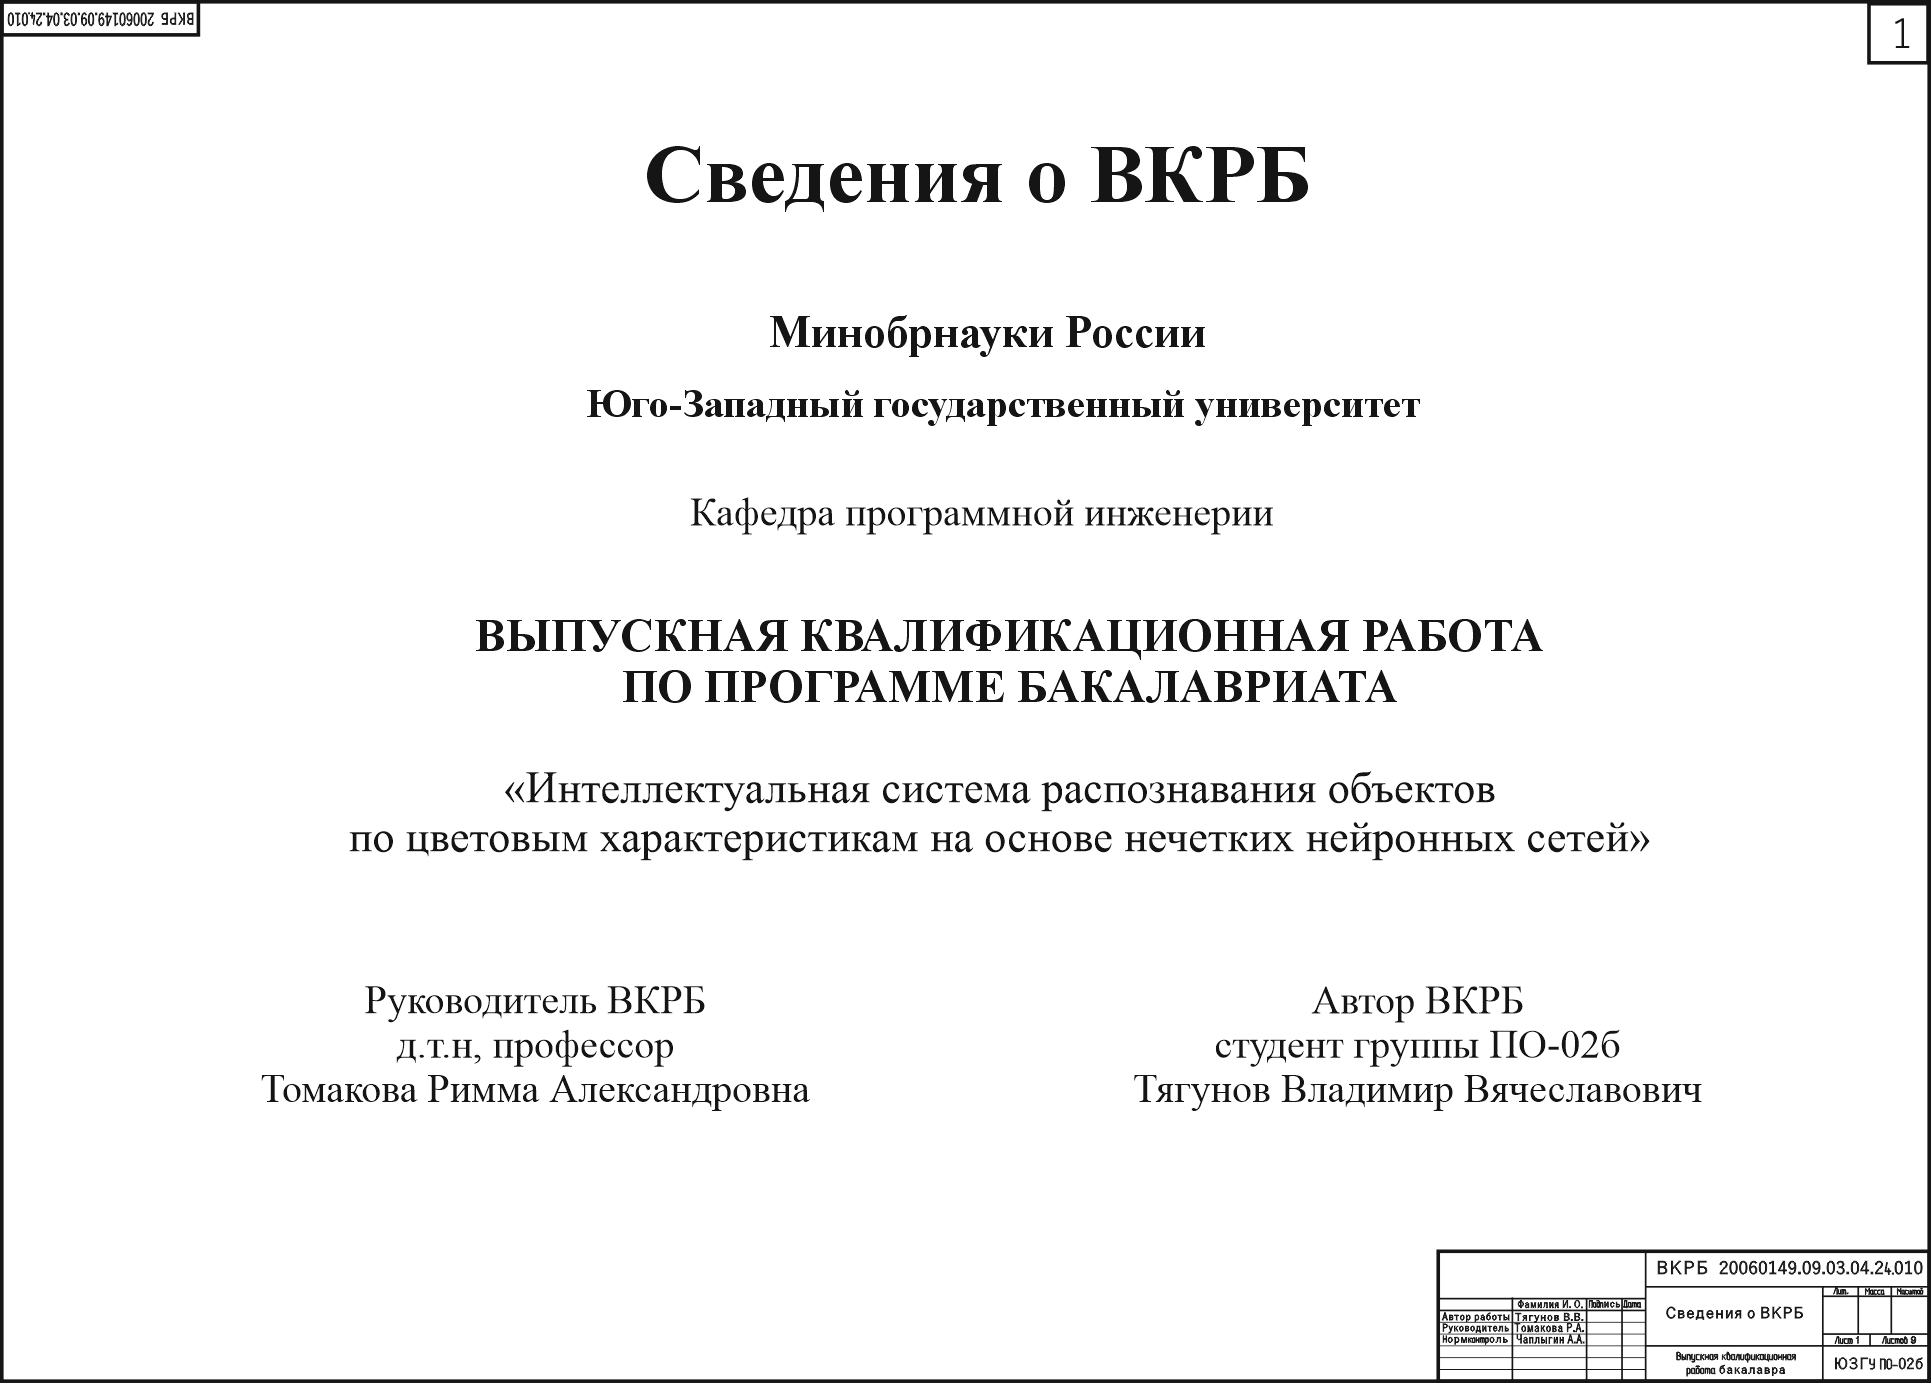
\includegraphics[width=0.82\linewidth]{Ramka_VKR}
    \заголовок{Сведения о ВКРБ}
    \label{Ramka_VKR:image}      
\end{плакат}

\begin{плакат}
    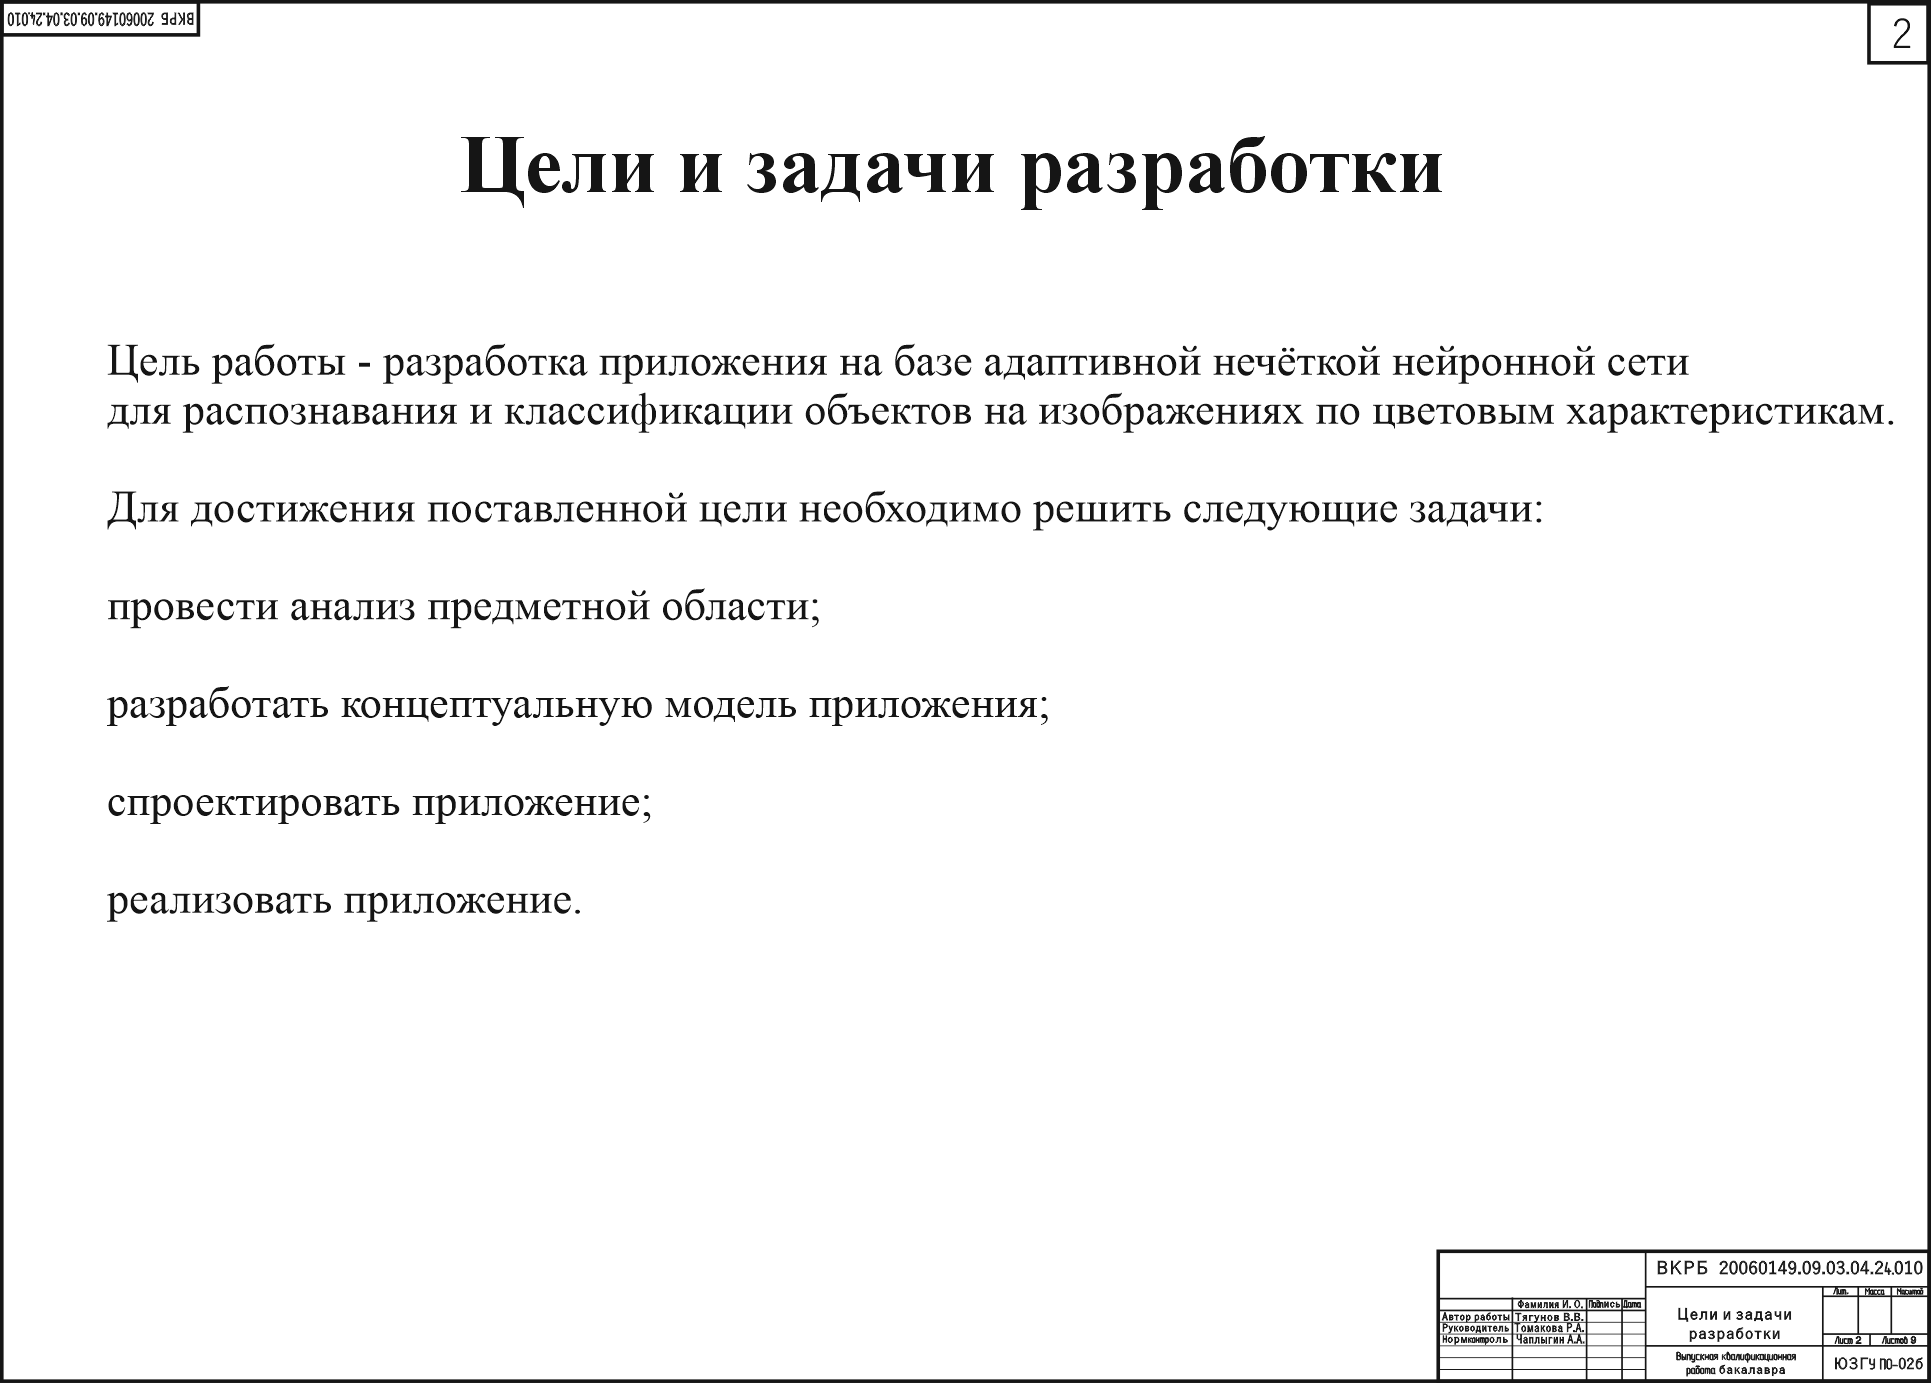
\includegraphics[width=0.82\linewidth]{Ramka_VKR2}
    \заголовок{Цель и задачи разработки}
    \label{Ramka_VKR2:image}      
\end{плакат}

\begin{плакат}
    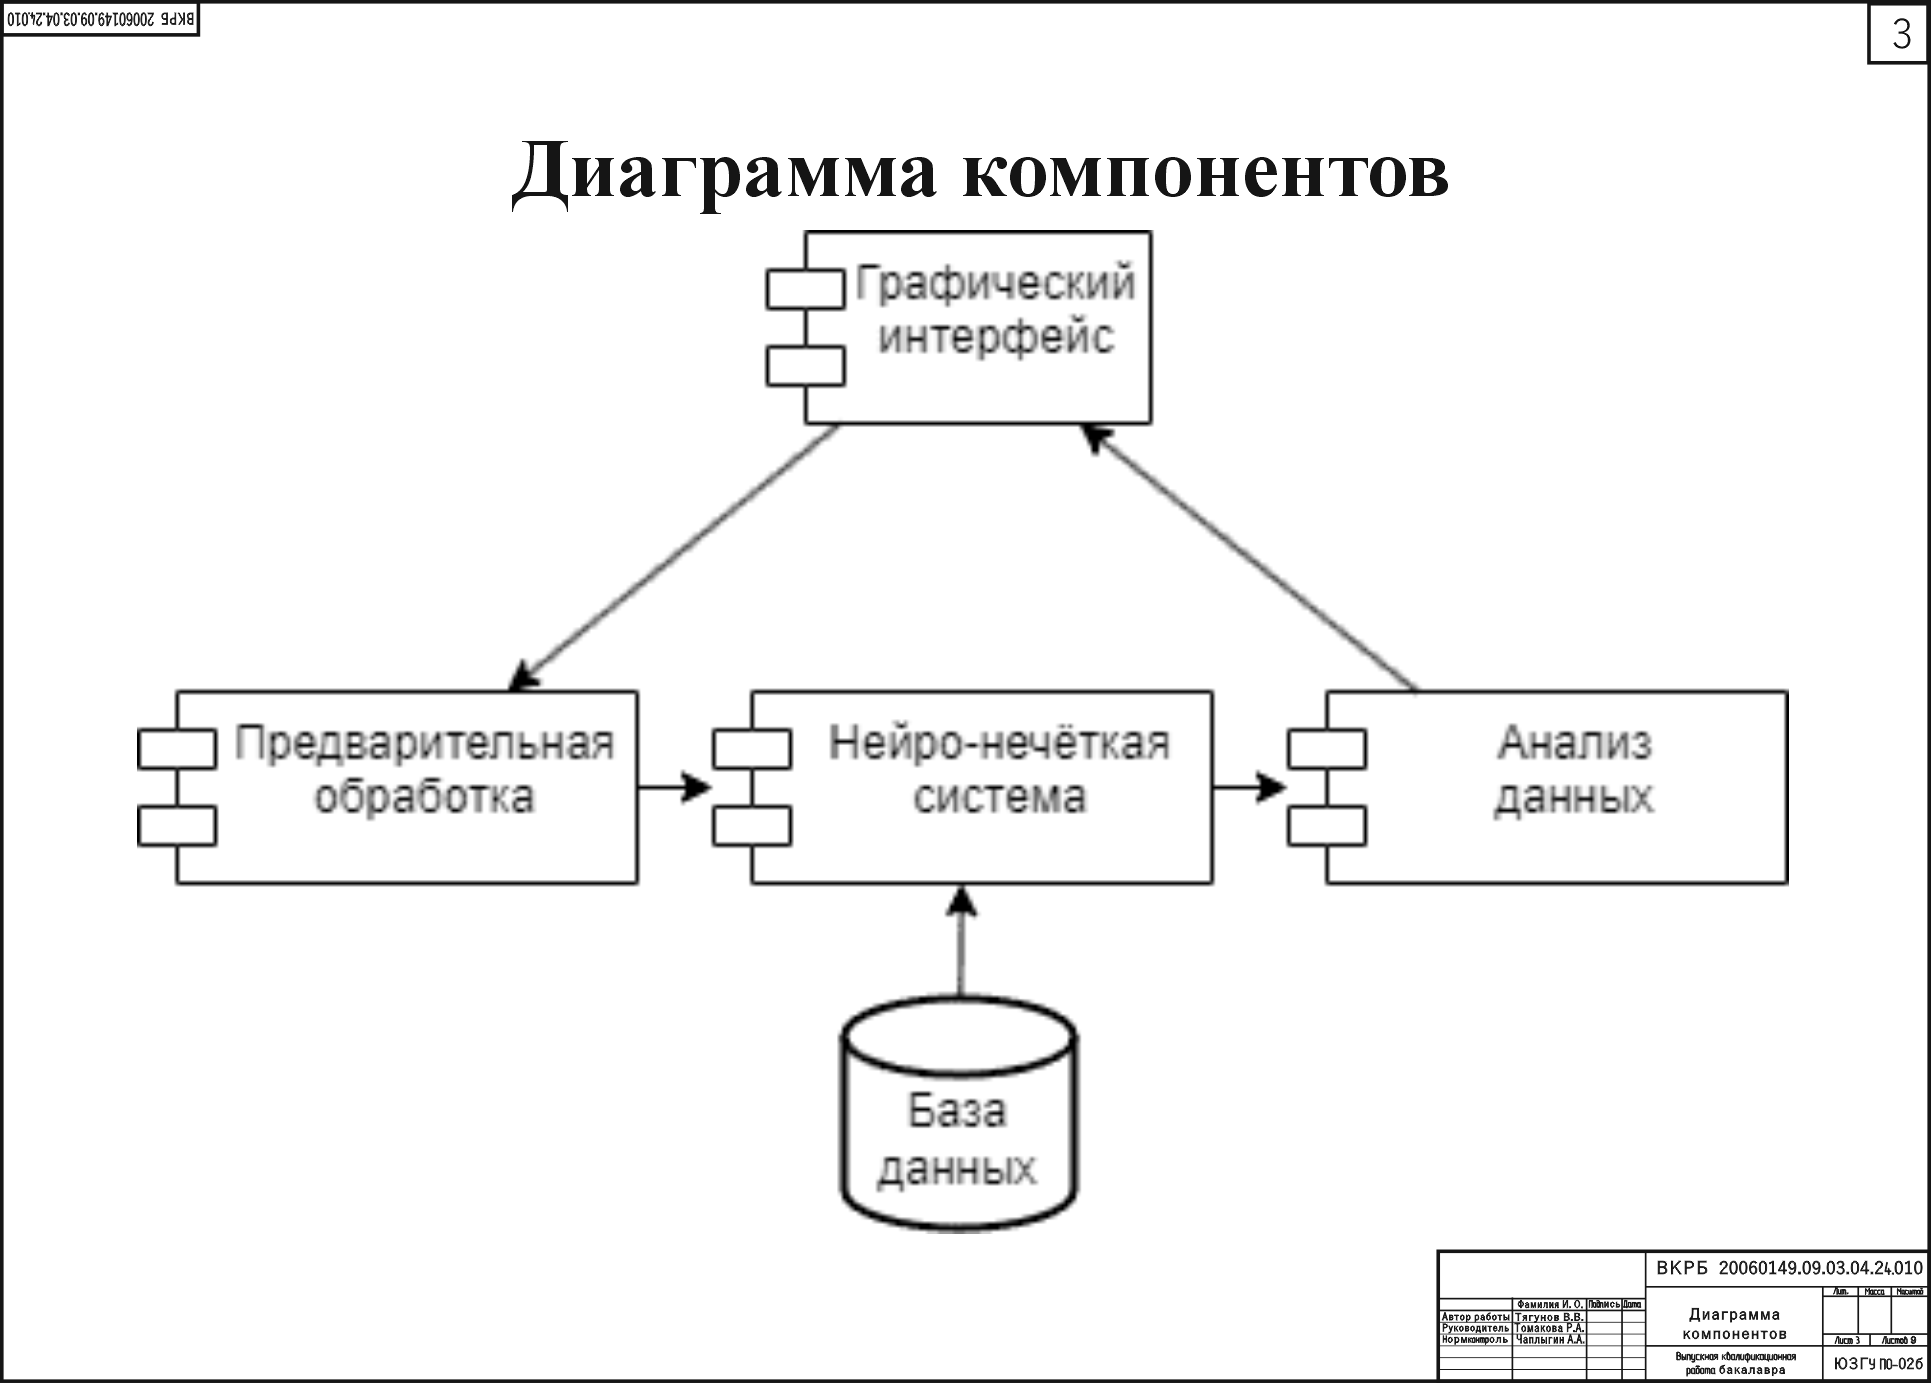
\includegraphics[width=0.82\linewidth]{Ramka_VKR3}
    \заголовок{Диаграммы компонентов}
    \label{Ramka_VKR3:image}      
\end{плакат}

\begin{плакат}
    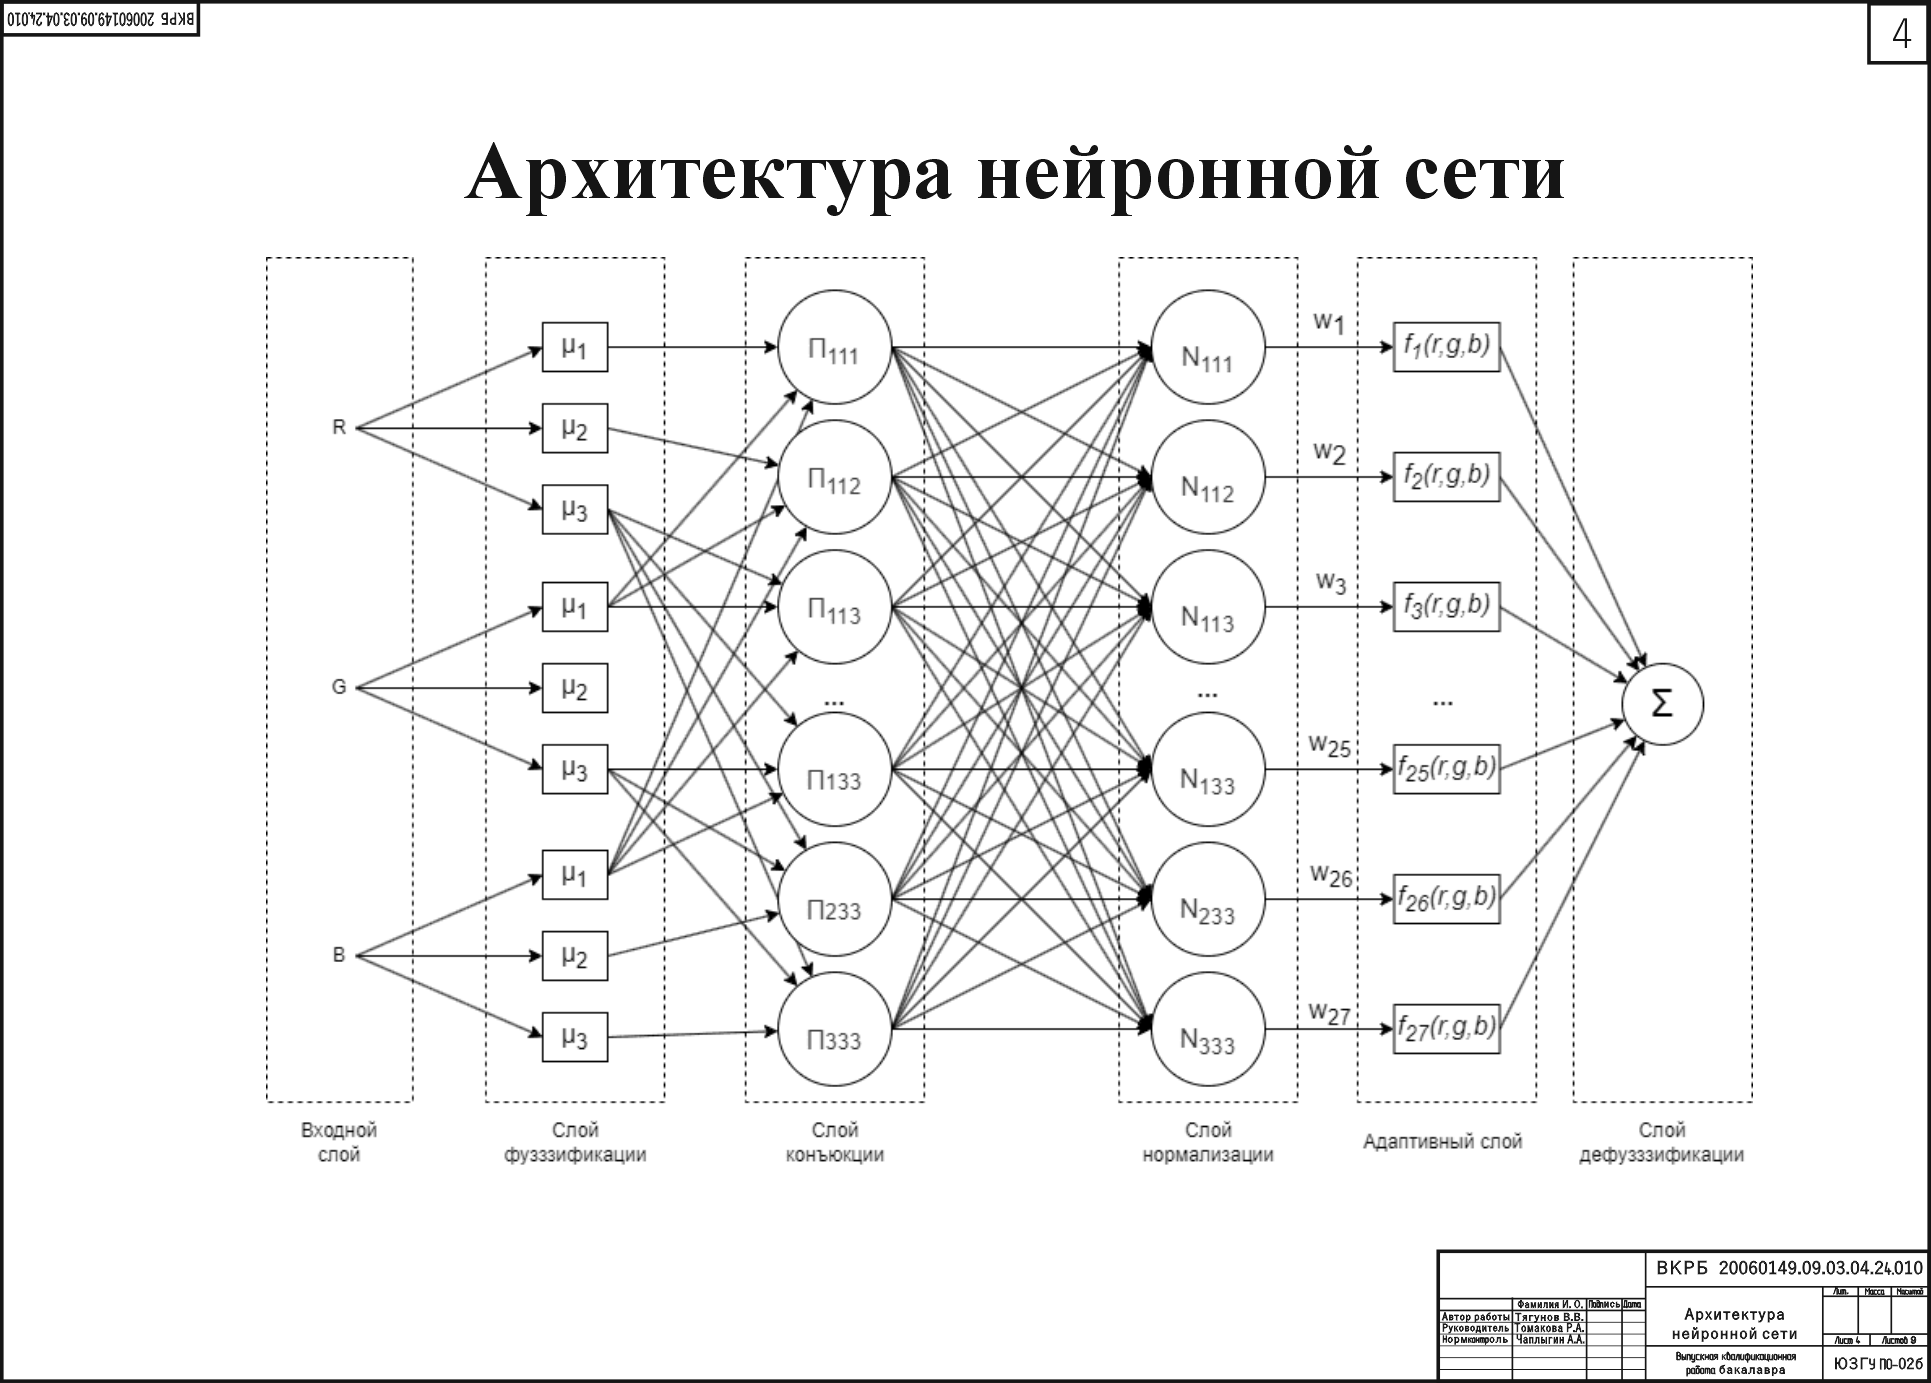
\includegraphics[width=0.82\linewidth]{Ramka_VKR4}
    \заголовок{Архитектура нейронной сети}
    \label{Ramka_VKR4:image}      
\end{плакат}

\begin{плакат}
    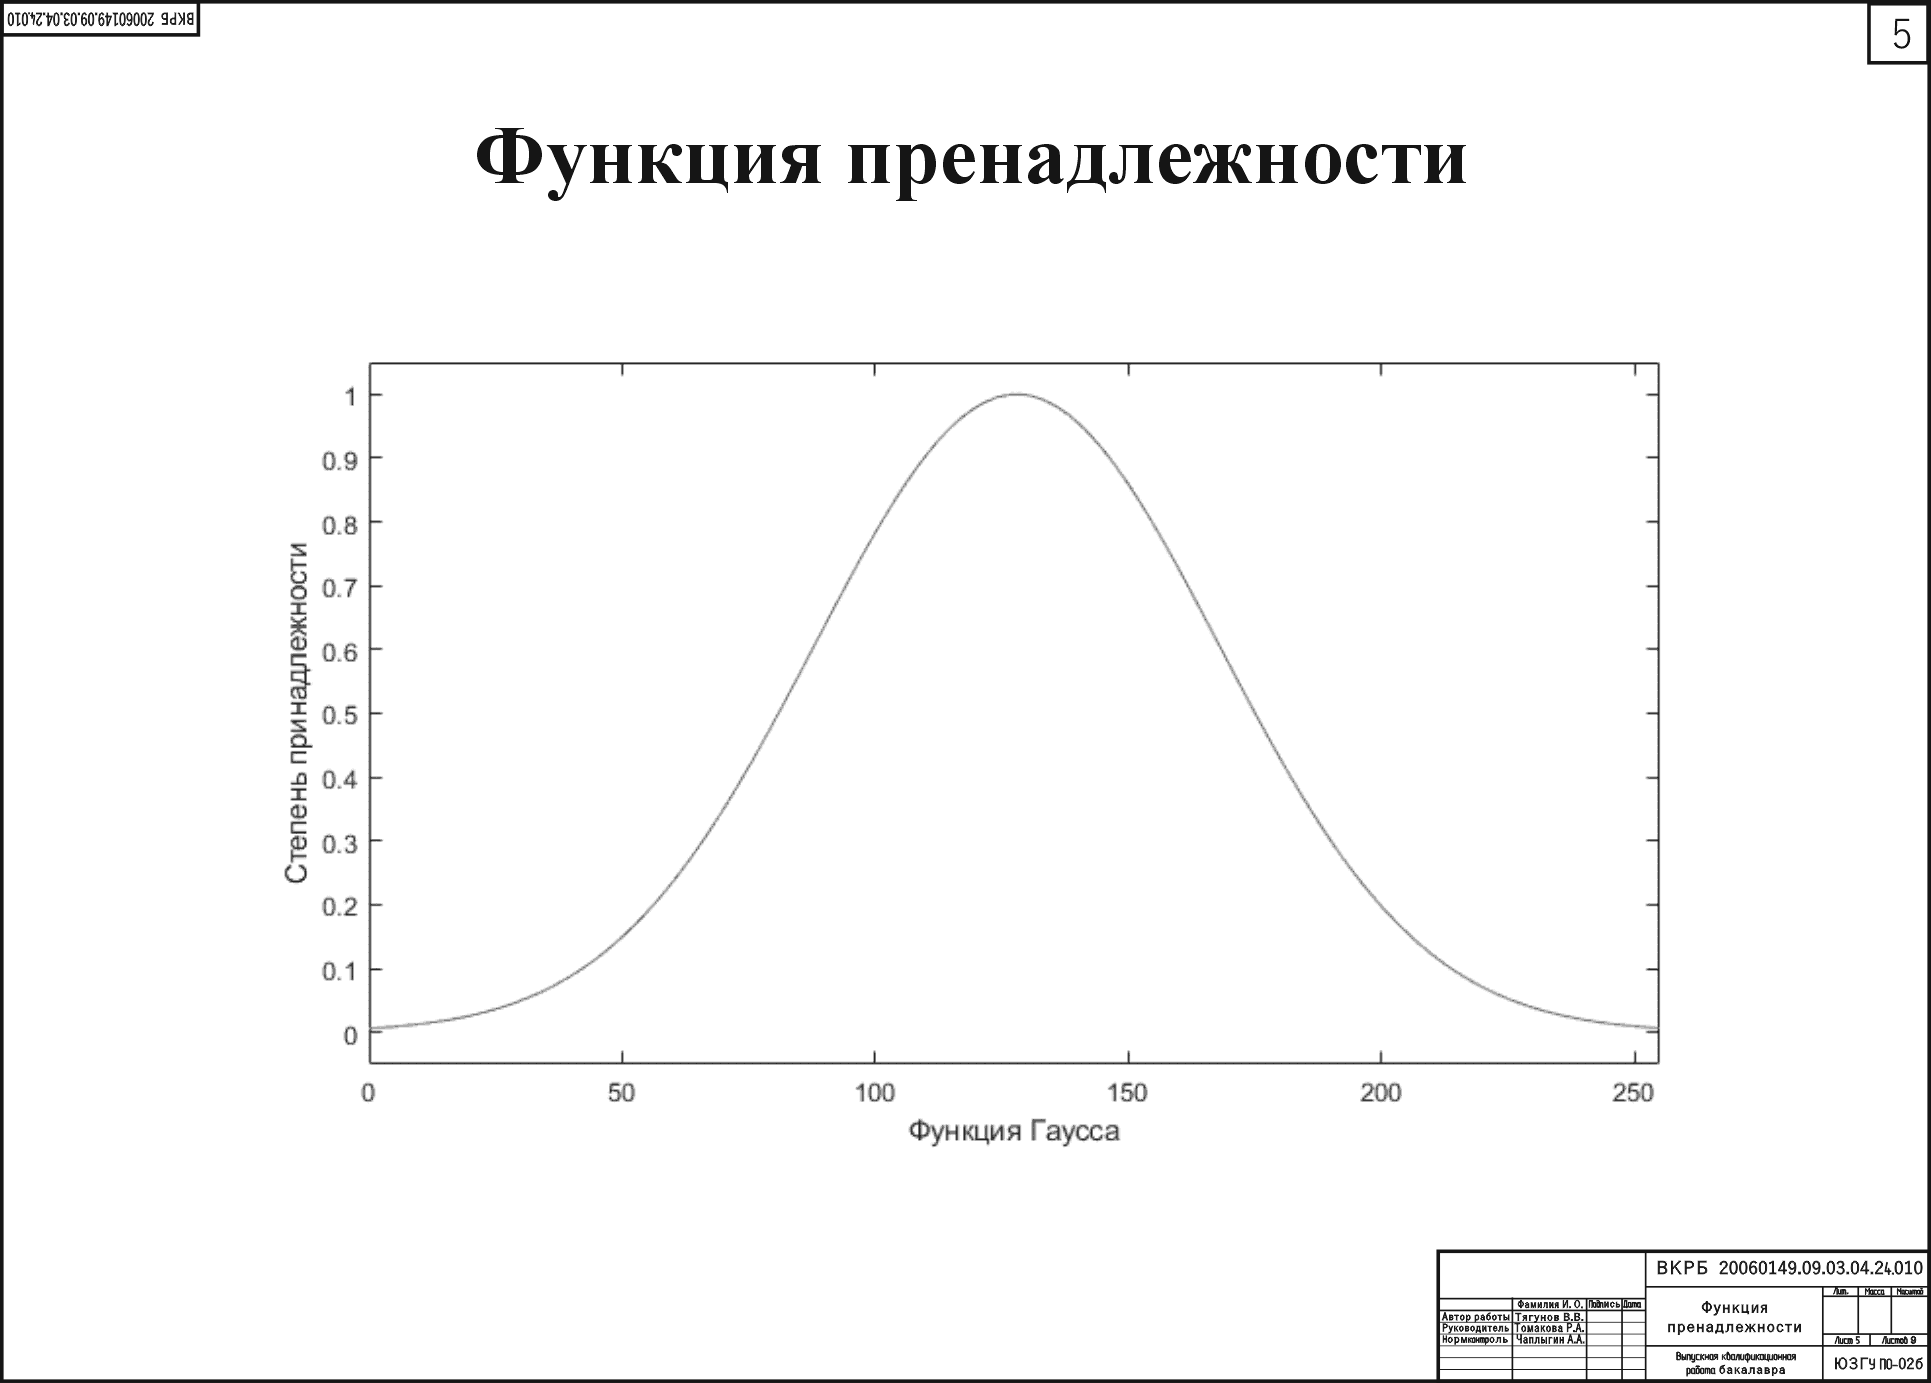
\includegraphics[width=0.82\linewidth]{Ramka_VKR5}
    \заголовок{Функция пренадлежности}
    \label{Ramka_VKR5:image}      
\end{плакат}

\begin{плакат}
    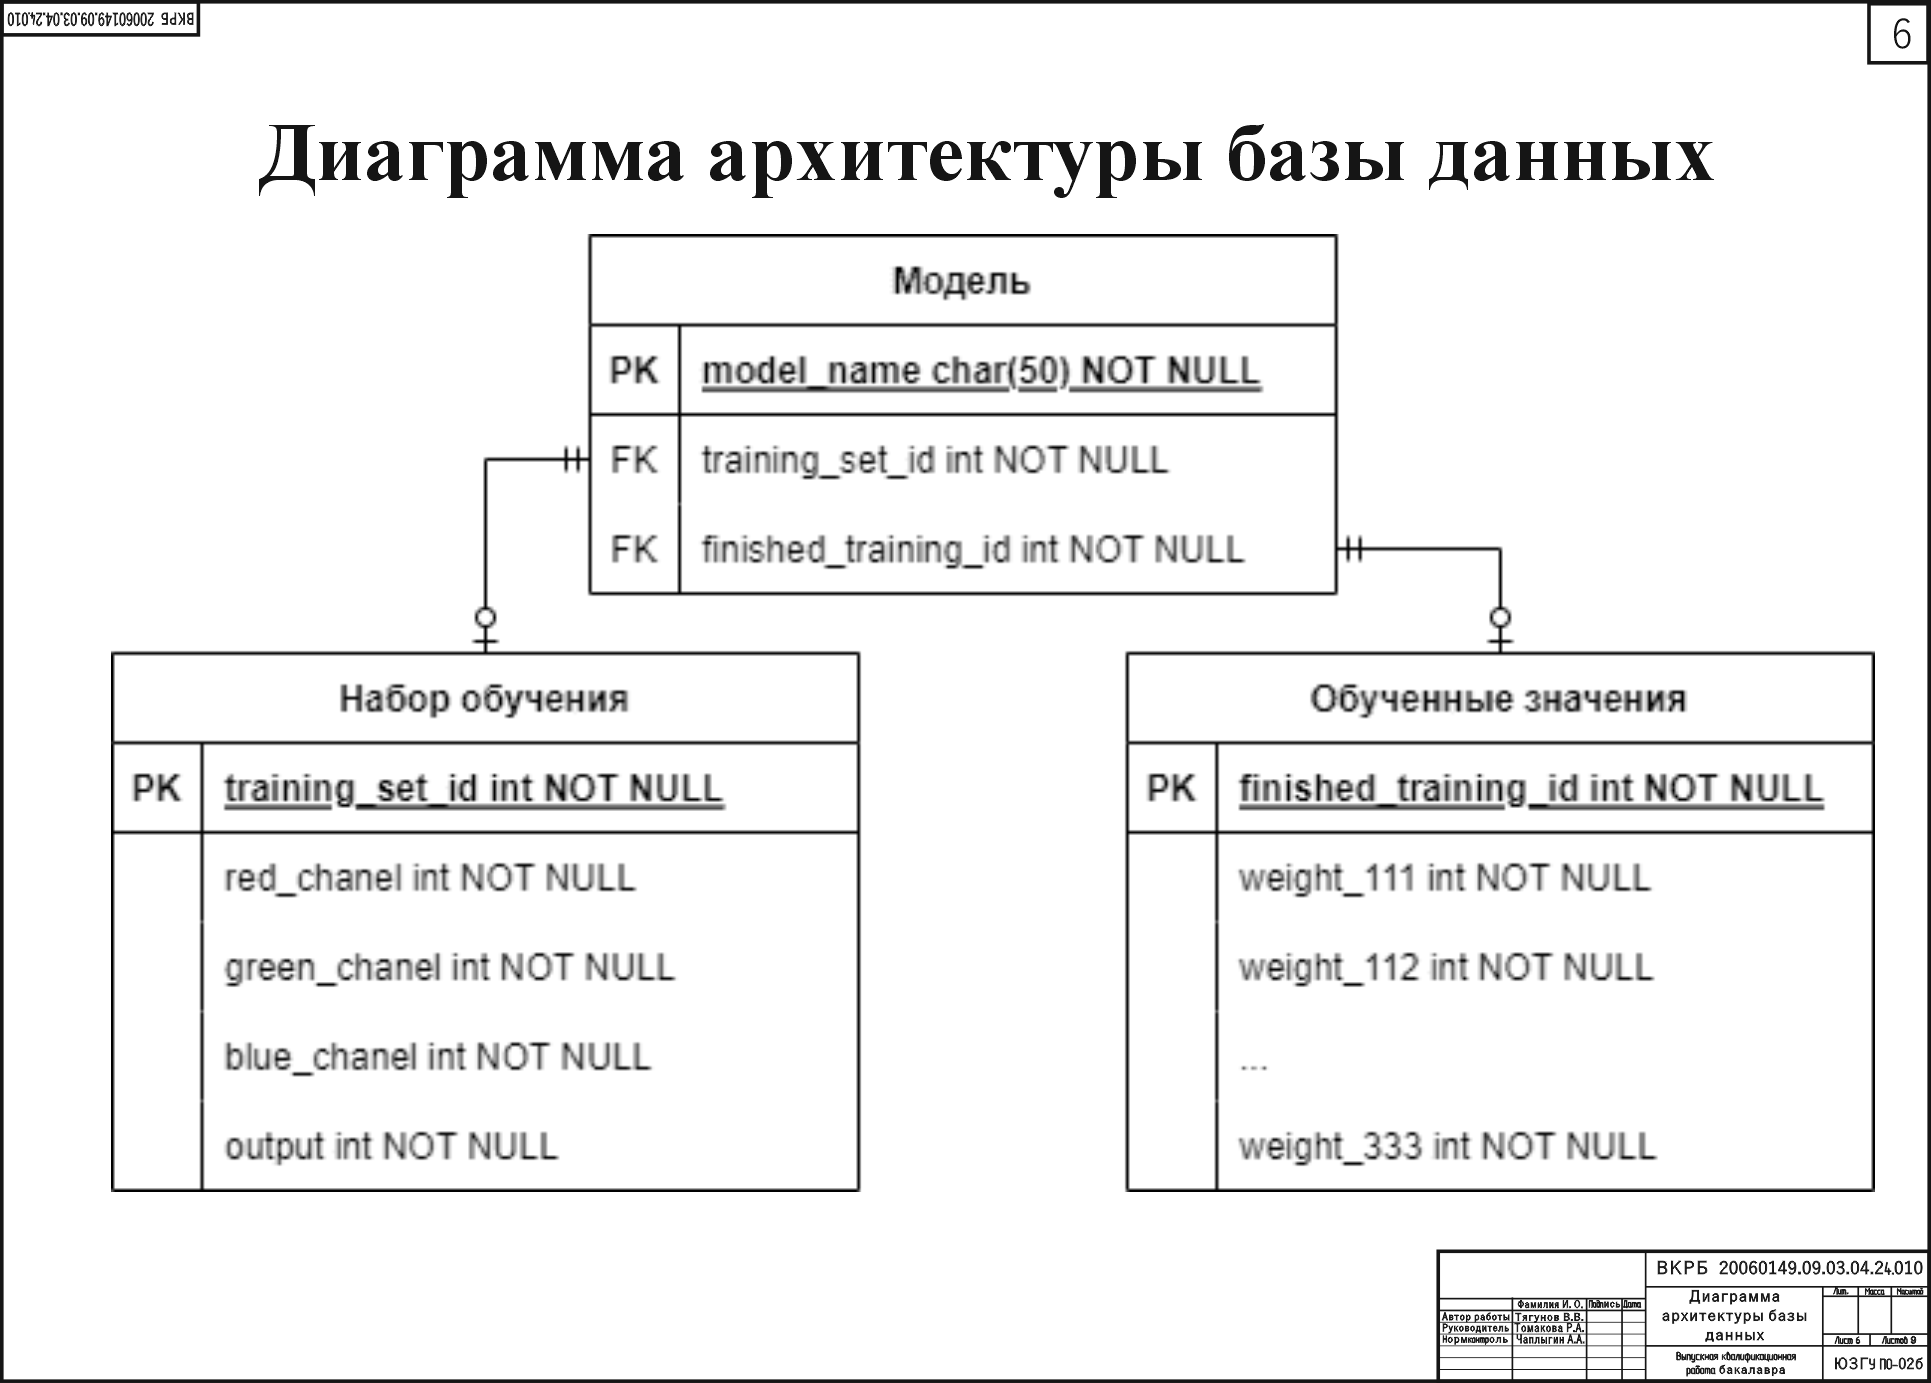
\includegraphics[width=0.82\linewidth]{Ramka_VKR6}
    \заголовок{База данных}
    \label{Ramka_VKR6:image}      
\end{плакат}

\begin{плакат}
    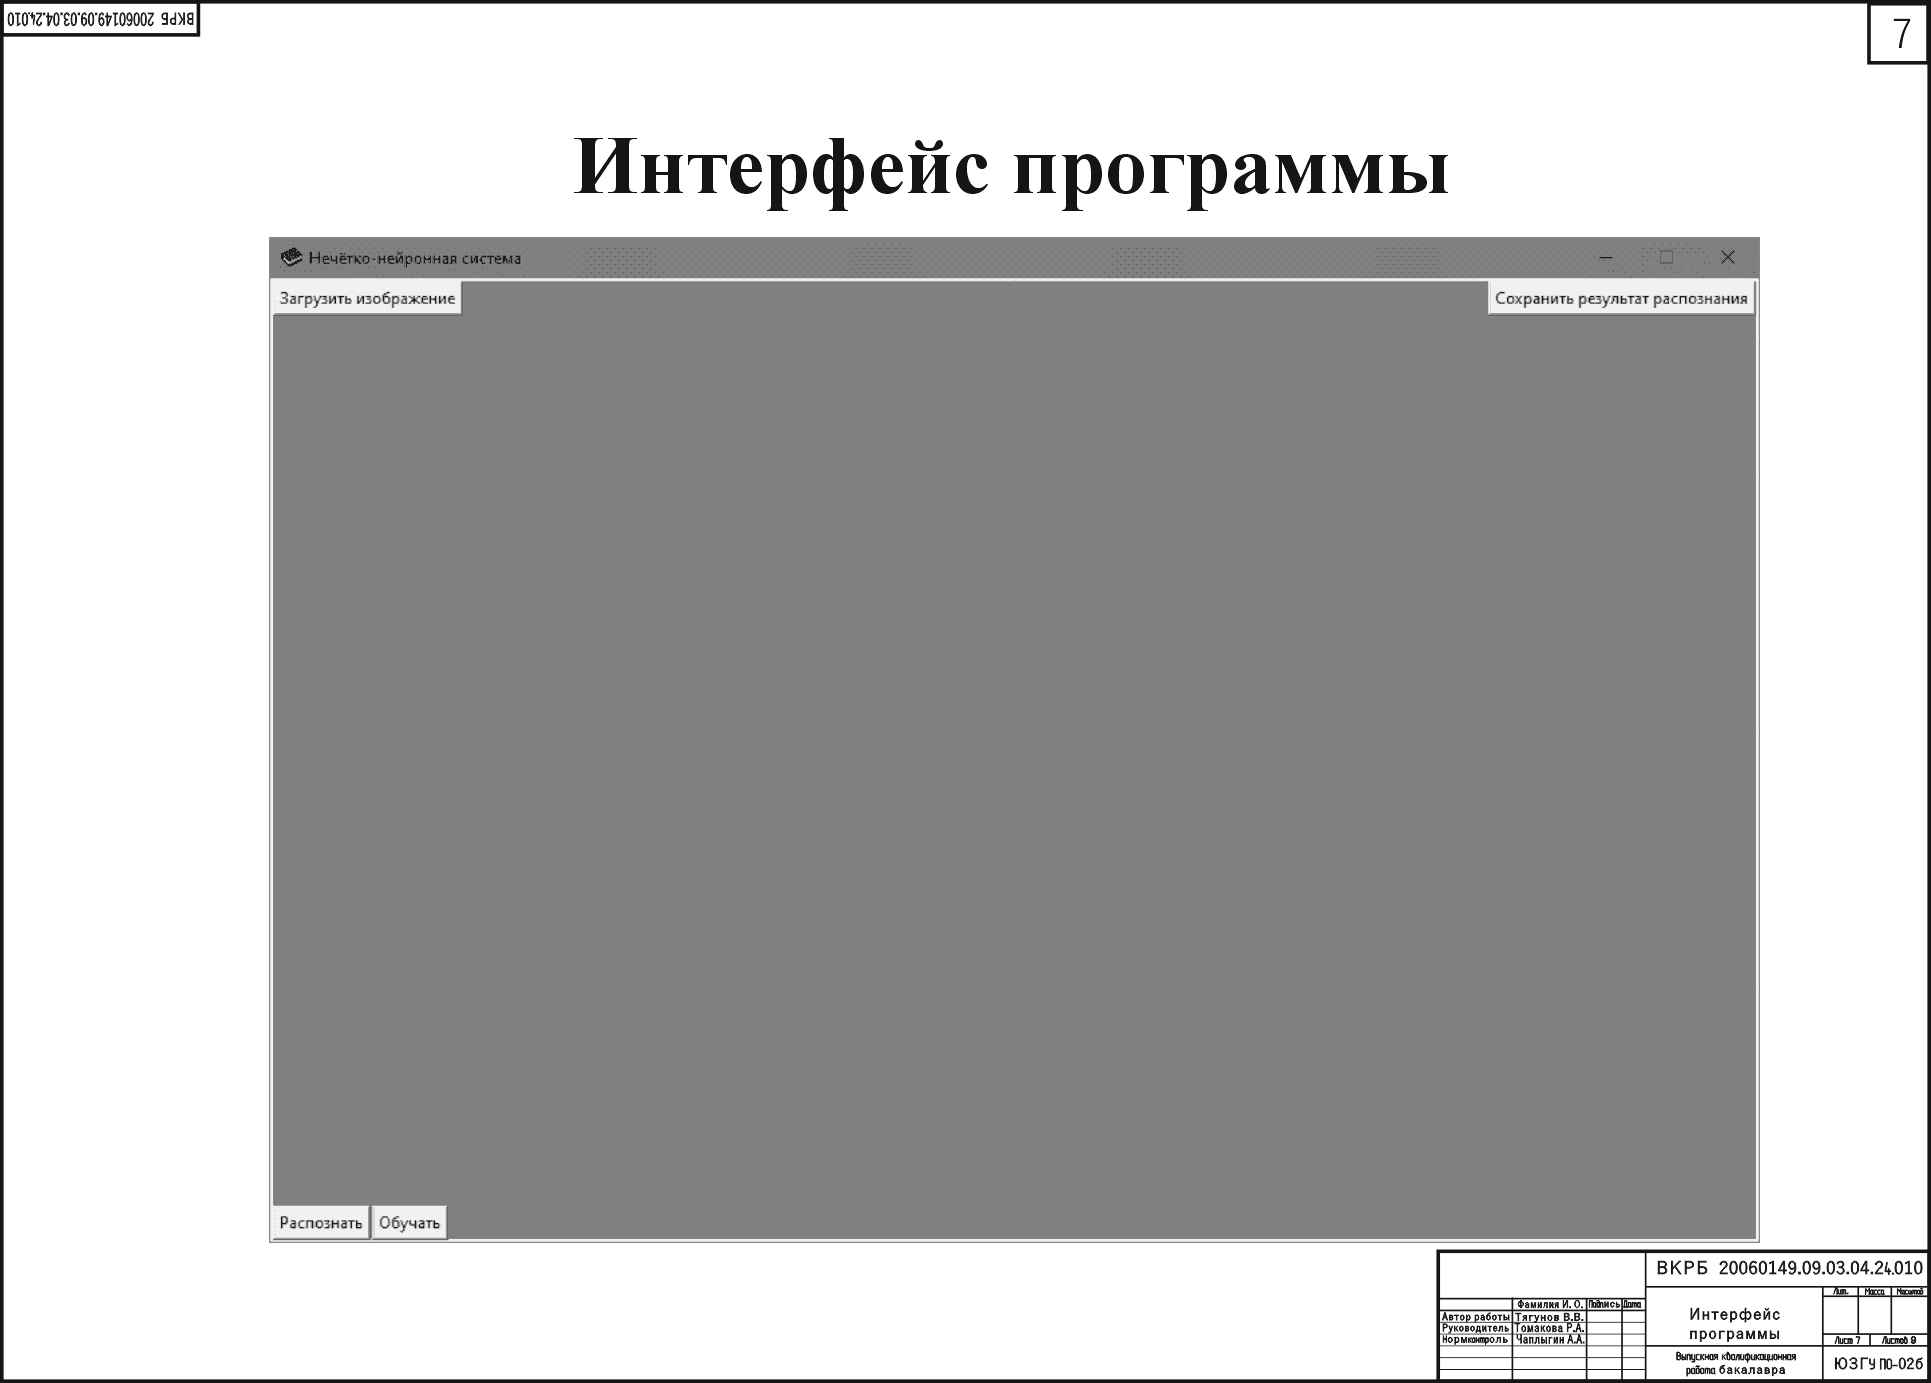
\includegraphics[width=0.82\linewidth]{Ramka_VKR7}
    \заголовок{Интерфейс приложения}
    \label{Ramka_VKR7:image}      
\end{плакат}

\begin{плакат}
    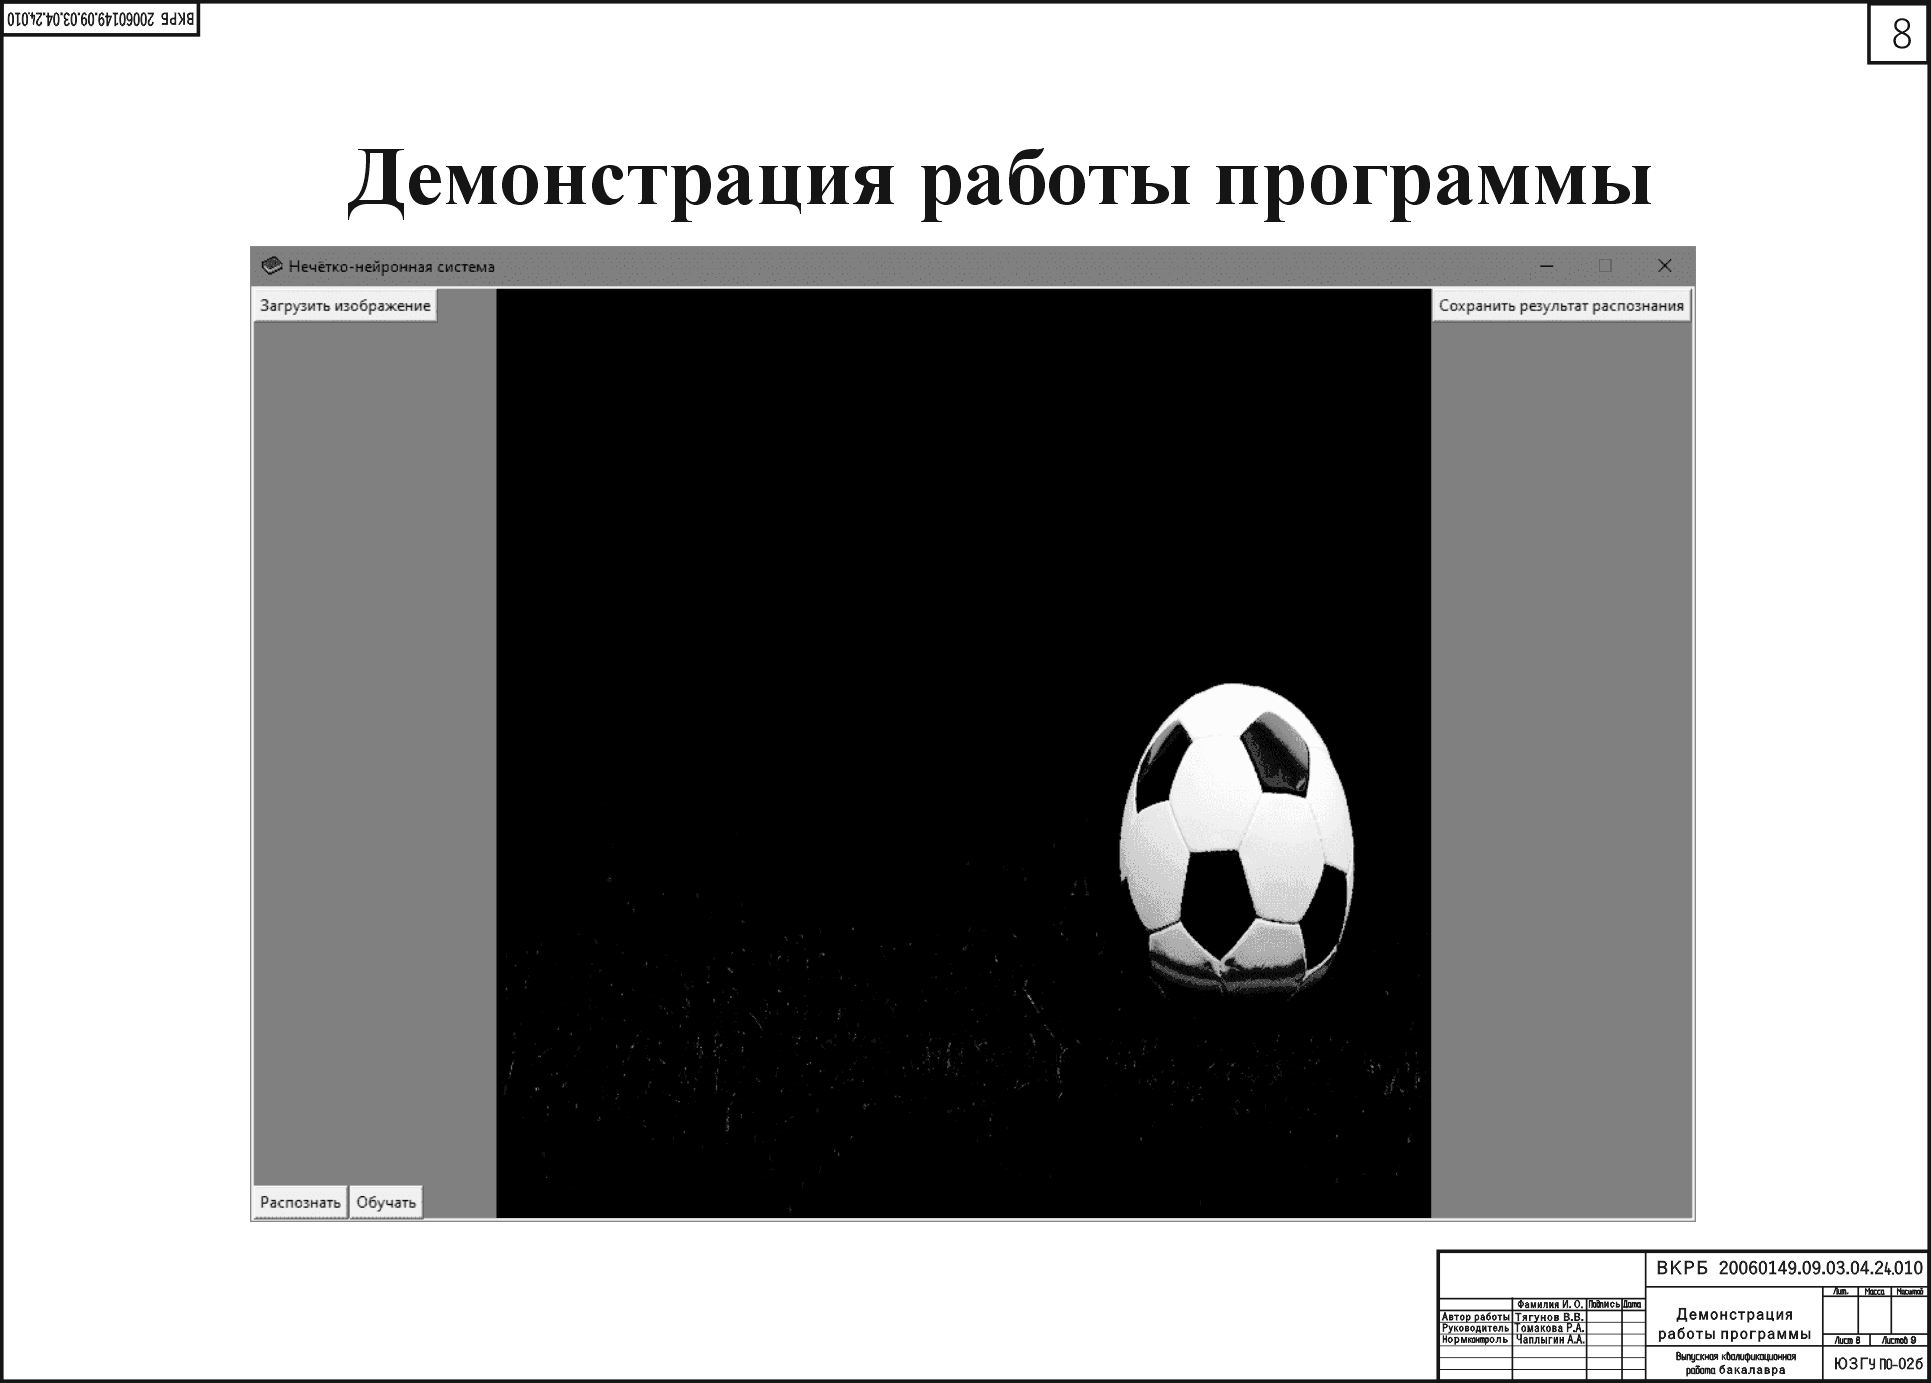
\includegraphics[width=0.82\linewidth]{Ramka_VKR8}
    \заголовок{Демонстрация работы программы}
    \label{Ramka_VKR8:image}      
\end{плакат}

\begin{плакат}
    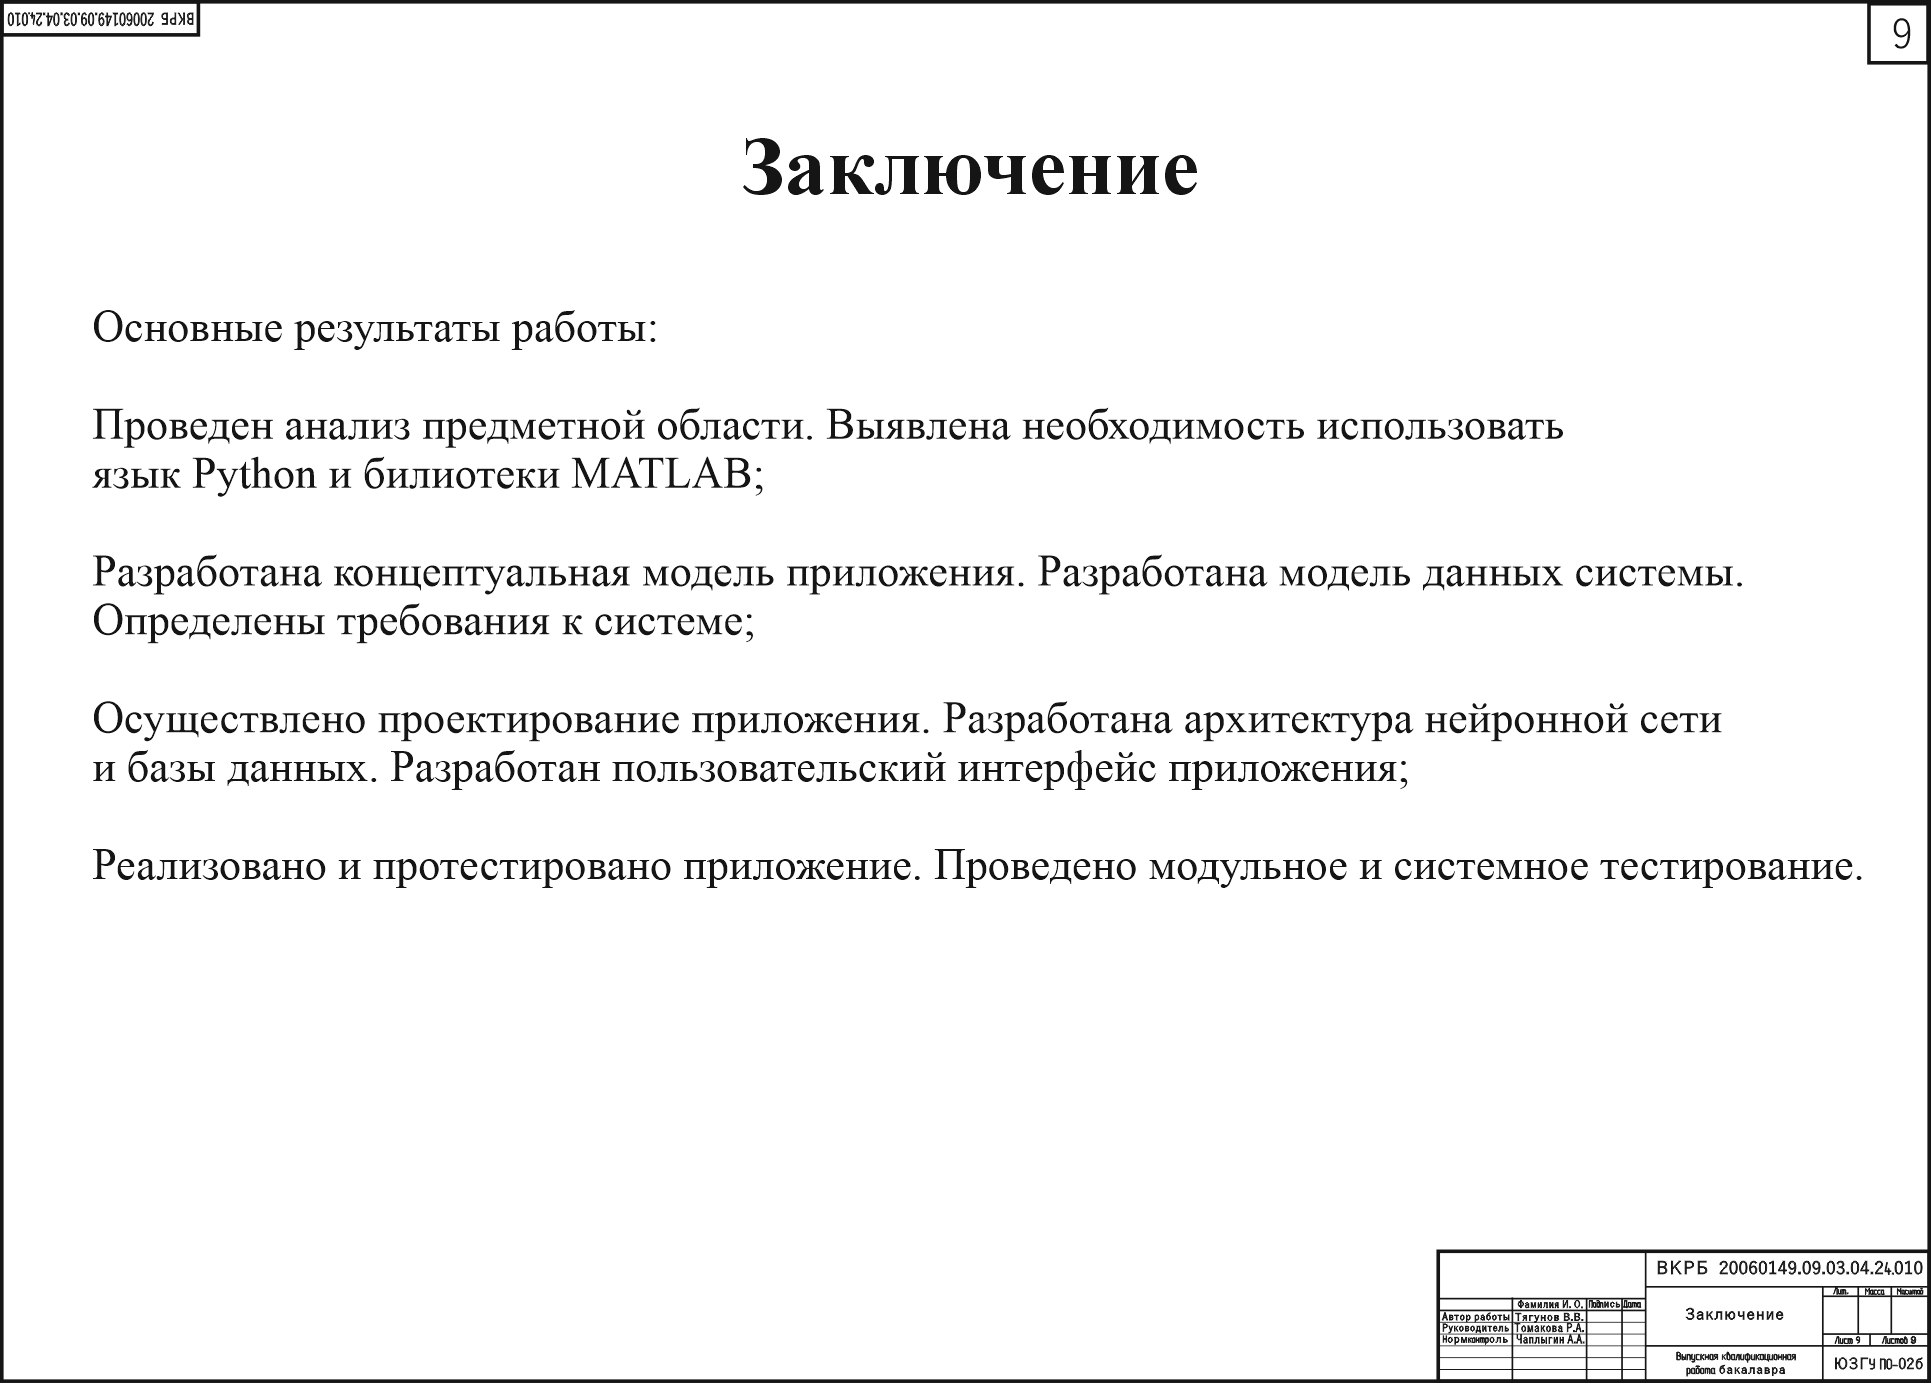
\includegraphics[width=0.82\linewidth]{Ramka_VKR9}
    \заголовок{Заключение}
    \label{Ramka_VKR9:image}      
\end{плакат}

\end{landscape}
